% Used Template for Computer Science Tripos Part II project dissertation, by Martin Richards, Simon Moore
\documentclass[12pt,a4paper,twoside,openright]{report}
\usepackage[pdfborder={0 0 0}]{hyperref}    % turns references into hyperlinks
\usepackage[margin=25mm]{geometry}  % adjusts page layout
\usepackage{graphicx}  % allows inclusion of PDF, PNG and JPG images
\usepackage{verbatim}
\usepackage{docmute}   % only needed to allow inclusion of proposal.tex
\usepackage{amsfonts}
\usepackage{amsmath}
\usepackage{tikz}
\usepackage{float}
\usepackage{cleveref}

\renewcommand{\vec}[1]{\mathbf{#1}}

\crefformat{section}{\S#2#1#3} % see manual of cleveref, section 8.2.1
\crefformat{subsection}{\S#2#1#3}
\crefformat{subsubsection}{\S#2#1#3}

\crefformat{figure}{Figure~#2#1#3}

\newcommand{\R}{\mathbb{R}}

\raggedbottom                           % try to avoid widows and orphans
\sloppy
\clubpenalty1000%
\widowpenalty1000%

\renewcommand{\baselinestretch}{1.1}    % adjust line spacing to make
                                        % more readable

\begin{document}
\pagenumbering{gobble}

\bibliographystyle{unsrt}

%%%%%%%%%%%%%%%%%%%%%%%%%%%%%%%%%%%%%%%%%%%%%%%%%%%%%%%%%%%%%%%%%%%%%%%%
% Title


\thispagestyle{empty}
\rightline{\Large\textbf{Ian Tai}}
\vspace*{50mm}
\begin{center}
\rule{\linewidth}{1pt}\vspace{5mm}
\LARGE\textbf{Learning the Stock Market: Deep Learning and Sentiment
Analysis-Based Stock Price Prediction}
\rule{\linewidth}{1pt} \\[10mm]
\Large\textsc{Computer Science Tripos -- Part II \\[5mm]
Trinity College \\[5mm]
\today}  % today's date
\end{center}

%%%%%%%%%%%%%%%%%%%%%%%%%%%%%%%%%%%%%%%%%%%%%%%%%%%%%%%%%%%%%%%%%%%%%%%%%%%%%%
% Proforma, table of contents and list of figures
\pagestyle{plain}
\setcounter{page}{1} 
\chapter*{Proforma}
\pagenumbering{roman}
{\large
\begin{tabular}{ll}
Name:               & \bf Ian Tai                      \\[-2pt]
College:            & \bf Trinity College                     \\[-2pt]
Project Title:      & \bf Learning the Stock Market: Deep Learning \\[-2pt]
& \bf and Sentiment Analysis-Based Stock Price\\[-2pt]
& \bf Prediction \\[-3pt]
Examination:        & \bf Computer Science Tripos Part II, May 2018  \\[-2pt]
Word Count:         & \footnotemark \\[-3pt]
Project Originator: & \bf Ian Tai                    \\[-2pt]
Supervisors:         & \bf Dr Sean Holden                    \\[-2pt]
& \bf Prof Stephen Satchell
\end{tabular}
}
\footnotetext[1]{This word count was computed
by \TeX count}

\stepcounter{footnote}


\section*{Original Aims of the Project}

Deep Learning has increasingly been applied to many fields of industry. Among Finance,
the applications of Deep Learning in predicting stock market prices is an increasingly
popular research field. This dissertation proposes a method of stock price prediction
using a combination of Long Short-Term Memory Recurrent Neural Networks and a variety
of Sentiment Analysis techniques. The project aims to apply this method to collected 
news headlines from selected news agencies on Twitter and stock price data from the 
latter two quarters of 2017.

\section*{Work Completed}

This project has been successful; all success criteria have been met. I collected, parsed, and converted
financial data from a Bloomberg Terminal. I 
built a data collection and processing system for the Twitter dataset. I implemented
Gaussian and Multinomial Naive Bayes Classifiers, and used the
Scikit-Learn library for implementing Multi-Class Support Vector Machines and
Semi-Supervised Support Vector Machines for sentiment analysis. Finally, I built
a Long Short-Term Memory Recursive Neural Network for stock price prediction. The techniques
proposed for predicting stock market prices have resulted in statistically significant results,
and may benefit financial and machine learning research in this field.

\section*{Special Difficulties}

Finding appropriate Twitter datasets proved to be more difficult than was foreseen, which led to
trying various sources of data, different models of classification, and ultimately, manual classification
of the data for train/test purposes.
 
\newpage
\section*{Declaration}

I, Ian Tai of Trinity College, being a candidate for Part II of the Computer
Science Tripos, hereby declare
that this dissertation and the work described in it are my own work,
unaided except as may be specified below, and that the dissertation
does not contain material that has already been used to any substantial
extent for a comparable purpose.

\bigskip
\leftline{Signed: Ian Tai}

\medskip
\leftline{Date: \today}

\tableofcontents

\listoffigures

\newpage
\section*{Acknowledgements}

I would like to thank the following people for the help they have given me:

TODO: COMPLETE AFTERWARDS

%%%%%%%%%%%%%%%%%%%%%%%%%%%%%%%%%%%%%%%%%%%%%%%%%%%%%%%%%%%%%%%%%%%%%%%
% now for the chapters

\pagestyle{headings}

\chapter{Introduction}

\pagenumbering{arabic}
TODO: Beginning Starting Intro

This dissertation describes the implementation, fusion, and testing of several Machine Learning (ML)
techniques for stock price prediction. Multinomial Naive Bayes, Gaussian Naive Bayes, and Multi Class
Support Vector Machines, using different methods of feature extraction, were used to classify the
sentiment of relevant Twitter posts of news headlines. The Long Short-Term Memory (LSTM) Recurrent 
Neural Network (RNN) was used for predicting stock prices, utilizing both
financial technical indicators and the output of the sentiment classifiers.


\section{Motivation \& Aims}

Under the Efficient Market Hypothesis, an efficient capital market fully reflects
all relevant information in determining security prices \cite{Malkiel89}. Since all past prices and
information are available to the market, it follows that correct predictions, if possible, will be immediately
taken advantage of, and the resulting market adjustment quickly nullifies any possible advantage. Thus,
it follows that an efficient market is unpredictable, and behaves in the manner of a Random Walk.

However, several factors contribute to potential inefficiency in practical markets --
there usually exists some latency in market information availability and absorption, varying liquidity levels
of different commodities and equities, different levels of information availability, and countless other
real-life factors. Thus, it is argued that there exists a window for prediction. [Cite several of these studies]

The wealth of available data regarding financial markets makes it a prime target for Machine Learning.



\section{Challenges}



\section{Related Work}



\chapter{Preparation}

This chapter includes all of the work that was completed before implementation began.
This includes the theory behind each Machine Learning model (\cref{sec:introNN},
\cref{sec:introSVM}, and \cref{sec:introNB}), financial
theory (\cref{sec:introFin}), feature extraction (\cref{sec:introFeat}), 
an outline of the project's requirements (\cref{sec:introReq}), tools and libraries
considered and used (\cref{sec:introTool}), development model (\cref{sec:introSoft}),
an early outline for implementation (\cref{sec:introImpl}), and the starting point
for my project (\cref{sec:introStart})

\section{Neural Networks}
\label{sec:introNN}

The theory regarding Recursive Neural Networks and
Long Short-Term Memory Networks in this section is adapted from \cite{Goodfellow-et-al-2016}.

\subsection{Introduction}

Before delving into Recurrent Neural Networks (RNNs), we must first discuss
the basics of Machine Learning (ML). An ML algorithm is one that learns from
data. Mitchell (1997) provides a definition for learning:
"A computer program is said to learn from experience E with respect to some
class of tasks T and performance measure P, if its performance at tasks in T, as
measured by P, improves with experience E." \cite{Mitchell97} 

The use of a recurrent neural network in my project is in the manner of
supervised learning. Supervised learning is a subset of Machine Learning,
where all given data is labelled, such that each input feature vector $\vec{x} \in \R^m$
is associated with a label $y$. This label can either be a discrete variable where 
$y \in C = [C_1, C_2, C_3, ..., C_n]$,
in the case of classification, or a continuous variable where $y \in \R$, in the case of regression.
The use of RNNs in this project is limited to regression.

A supervised learning algorithm for regression, given a training sequence
\begin{equation}
\vec{s} = ((\vec{x_1}, y_1), (\vec{x_2}, y_2), (\vec{x_3}, y_3), ... , (\vec{x_n}, y_n))
\end{equation}

where $(\vec{x_1}, y_1)$ is a training input, learns a function $h: \R^m \rightarrow \R$,
a hypothesis, that approximates a match between an input feature vector $\vec{x}$ to a
result $y$.

After learning this hypothesis function, the algorithm can then be used to predict test
samples $\vec{x'}$. We can then run accuracy measurements and goodness-of-fit tests on
the resulting outputs, given we know the original labels $y'$.

\subsection{Artificial Neurons}

A neural network is a network of artificial neurons that each takes an input $\vec{x}$,
and runs a linear combination of the input feature vector $\vec{x}$, weights $\vec{w}$, and a bias $b$,
fed through an activation function $\sigma$. The formulation is detailed below:

\begin{equation}
y = \sigma (\vec{wx} + b)
\end{equation}

The activation function is used to ensure the output stays within a preset bound,
usually either $[0,1]$ or $[-1,1]$. Typical activation functions are as follows:
\begin{align}
\intertext{Logistic Function (Sigmoid):}
&\sigma(x) = \frac{1}{1+e^{-x}}\\
\intertext{Rectified Linear Unit (RELU):}
&\sigma(x) = \text{max}(0,x)\\[10pt]
\intertext{Hyperbolic Tangent (tanh):}
&\sigma(x) = \frac{e^x - e^{-x}}{e^x + e^{-x}}
\end{align}\\*

\begin{figure}[h]
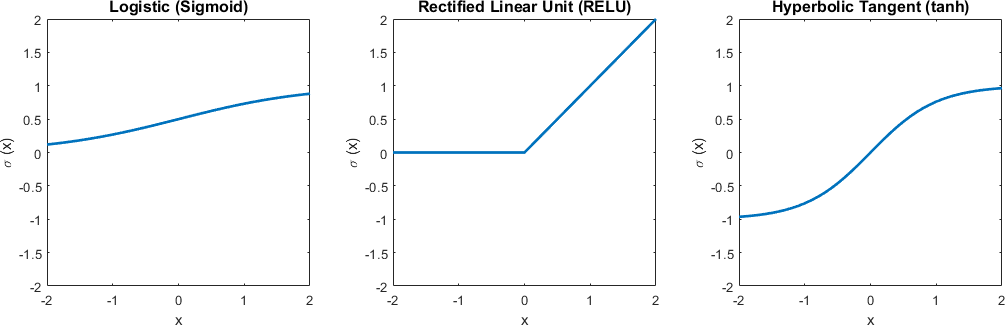
\includegraphics[width=\textwidth]{ActivationFunsCrop.png}
\caption{Plots of Sigmoid, RELU, and Hyperbolic Tangent functions}
\end{figure}

The output is then fed as either an input to other artificial neurons, or is the overall
output of the neural network.

\subsection{Training}
\label{sec:introTrain}

The training of the network using the training set first includes initialization of the 
weights and biases. Initialization will be covered in depth in the Implementation section
for the Long Short-Term Memory RNN (\cref{sec:ImplLSTM}).

For a basic NN, such as the Multi-Layer Perceptron (MLP), the output of the NN is
observed by simple \textbf{feed-forward propagation}. This means in the directed graph
of the NN architecture, calculated values for each training example ($\vec{x_i}$)
flow from neuron to neuron across layers, and the eventual
output is run through a final activation function to obtain the final result.

This output ($y_i'$) can then be fed into the \textbf{loss function} to calculate the error for this
training example. A typical loss function for this purpose is the Sum of Squared Errors 
function\footnote{Adapted from Dr Sean Holden's Machine Learning and Bayesian Inference Part II course \cite{Holden18}}:

\begin{equation}
\text{E}(\vec{x}, \vec{y}, \vec{w}, \vec{b})  = \sum_{i=1}^{n} (y_i - y_i')^2
\end{equation}

where $\vec{w}$ and $\vec{b}$ specify the weights and biases of the NN respectively, 
$\vec{x}$ is the set of training examples,
$\vec{y}$ is the set of training labels, n is the number of training examples, and $y_i$ and $y_i'$
are the training label and output value for training example $i$, respectively.

Based on the output of the loss function, the NN can then adjust its weights and biases to minimize
loss. This adjustment is performed using \textbf{gradient descent}. This optimization algorithm
iteratively updates these parameters using the gradients calculated from the loss function until
convergence is reached. Different variations of gradient descent used for the Long Short-Term Memory 
network (LSTM) will be discussed further in the Implementation section for LSTMs
(\cref{sec:ImplLSTM}).

The gradients are calculated as follows:
\begin{align}
\vec{w_{t+1}} &= \vec{w_t} - \lambda \frac{\delta E(\vec{x}, \vec{y}, \vec{w}, \vec{b})}{\delta \vec{w}} \Big|_\vec{w_t}\\
\vec{b_{t+1}} &= \vec{b_t} - \lambda \frac{\delta E(\vec{x}, \vec{y}, \vec{w}, \vec{b})}{\delta \vec{b}} \Big|_\vec{b_t}
\end{align}
where $\vec{w_{t+1}}$ and $\vec{b_{t+1}}$ are the weight and bias vectors at iteration $t$, respectively.
The parameter $\lambda$ is known as the learning rate, a hyperparameter\footnote{Hyperparameters are configurable
settings for a Neural Network that are often manually tuned for optimal performance and desired run-time} for NNs.
The learning rate must be chosen carefully; if it is too small, the NN may take an exceedingly long time to reach
convergence during the training period, and if too large, the NN may never find an appropriate minimum.

\begin{figure}[H]
\centering
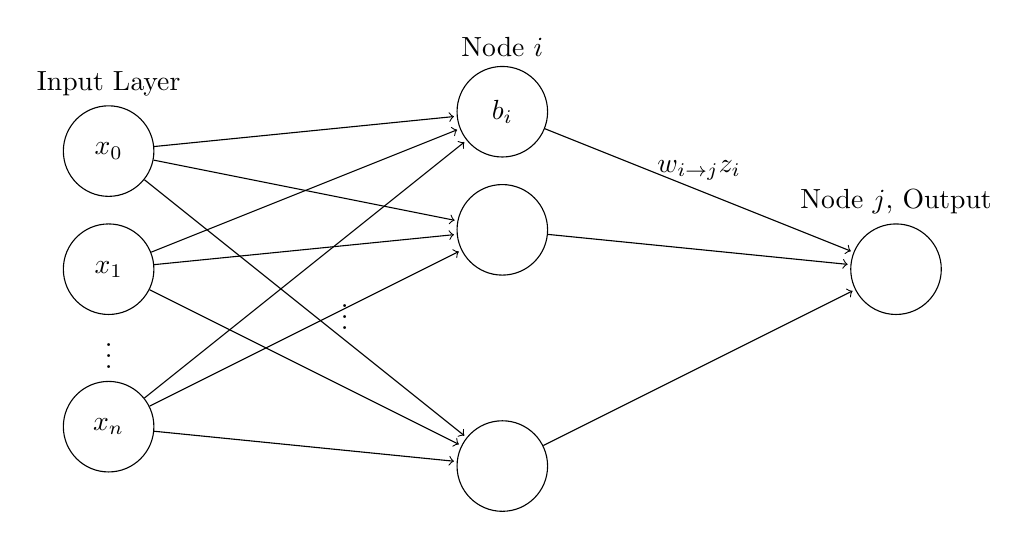
\begin{tikzpicture}[shorten >=1pt]
	\tikzstyle{unit}=[draw,shape=circle,minimum size=1.15cm]

	\node[label={Input Layer},unit](x0) at (0,3.5){$x_0$};
	\node[unit](x1) at (0,2){$x_1$};
	\node at (0,1){\vdots};
	\node[unit](xd) at (0,0){$x_n$};

	\node[label={Node $i$}, unit](h10) at (5,4){$b_i$};
	\node[unit](h11) at (5,2.5){};
	\node at (3,1.5){\vdots};
	\node[unit](h1m) at (5,-0.5){};

	\node[label={Node $j$, Output},unit](y2) at (10,2){};

	\draw[->] (x0) -- (h10);
	\draw[->] (x0) -- (h11);
	\draw[->] (x0) -- (h1m);
	
	\draw[->] (x1) -- (h10);
	\draw[->] (x1) -- (h11);
	\draw[->] (x1) -- (h1m);

	\draw[->] (xd) -- (h10);
	\draw[->] (xd) -- (h11);
	\draw[->] (xd) -- (h1m);

	\draw[->] (h10) -- (y2) node[midway, above] {$w_{i \rightarrow j} z_i$};

	\draw[->] (h11) -- (y2);

	\draw[->] (h1m) -- (y2);

\end{tikzpicture}
\caption[Layout of an MLP]{Layout of a Multi-Layer Perceptron\footnotemark}
\label{fig:MLP}
\end{figure}

\footnotetext{$w_{i \rightarrow j} z_i$ is the weight associated with the output
of node $i$ as the input to node $j$ multiplied by the output of node $i$, $z_i$. $b_i$ is the bias associated with node $i$.
Adapted from Dr Sean Holden's Artificial Intelligence I Part IB course \cite{Holden18AI1}}

The weights and biases at various levels of the NN are updated using \textbf{backpropagation}. Backpropagation
is the method used for calculating $\frac{\delta E(\vec{x}, \vec{y}, \vec{w}, \vec{b})}{\delta \vec{w}}$ and
$\frac{\delta E(\vec{x}, \vec{y}, \vec{w}, \vec{b})}{\delta \vec{b}}$ for every weight $w_{i \rightarrow j}$ and bias
$b_{i}$, as shown in \cref{fig:MLP}. This can be calculated directly, since the gradient at each node in a layer is
independent when the chain rule is applied, using the calculated gradients of any nodes that take the input from
node $j$. Thus, we apply backpropagation to find the gradient of each weight, starting from the output node and
working our way backwards until we reach the input feature vectors. This can be summarized into the following:

\begin{align}
\frac{\delta E(\vec{x}, \vec{y}, \vec{w}, \vec{b})}{\delta w_{i \rightarrow j}} &= z_i \sigma_j(a_j) \sum_k \delta_k w_{j \rightarrow k}\\
\intertext{\indent where}
a_j &= \sum_k w_{k \rightarrow j} z_k
\end{align}

where $k$ is any node that takes the output of node $j$, $z_i$ is the value output of node $i$,
$\sigma_j$ is the activation function for the node $j$,
and $\delta_k$ is the gradient for $w_{k \rightarrow j}$ that has already been calculated.
This formulation for calculating the weights' gradients can include the gradients for the bias, if we simply
label the bias as an extra weight, multiplied by an arbitrary $z = 1$. 

\subsection{Recurrent Neural Networks}
\label{sec:introRNN}

\begin{figure}[H]
\centering
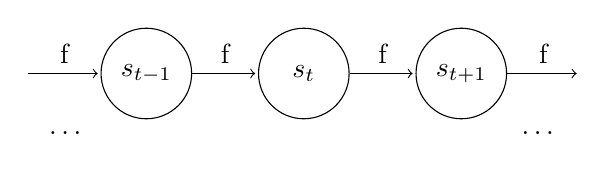
\begin{tikzpicture}[shorten >=1pt]
	\tikzstyle{unit}=[draw,shape=circle,minimum size=1.15cm]
	
	
	\node at (5,2.75){\dots};
	
	\node[unit](h0) at (6,3.5){$s_{t-1}$};
	\node[unit](h1) at (8,3.5){$s_{t}$};
	\node[unit](h2) at (10,3.5){$s_{t+1}$};
	
	\node at (11,2.75){\dots};
	
	\draw[->] (4.5,3.5) -- (h0) node[midway, above] {f};
	\draw[->] (h0) -- (h1) node[midway, above] {f};
	\draw[->] (h1) -- (h2) node[midway, above] {f};
	\draw[->] (h2) -- (11.5,3.5) node[midway, above] {f};
	
\end{tikzpicture}
\caption[States of a Dynamic System]{The evolution of state in a system\footnotemark}
\label{fig:seqIn}
\end{figure}

Feed-forward networks require that each training example be input into the network in full, and that
each example be independent of each other. If we have the case of sequentially dependent inputs,
such as the state of a dynamic system that evolves with regards to a time $t$ (\cref{fig:seqIn}), then we can use
a Recurrent Neural Network.

\footnotetext{Each node represents the state at
some time $t$, which is mapped according to some underlying function f, to the state at time $t+1$}

\begin{figure}[H]
\centering
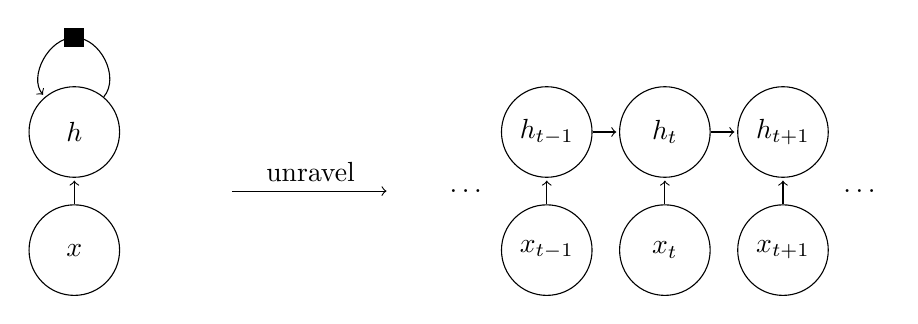
\begin{tikzpicture}[shorten >=1pt]
	\tikzstyle{unit}=[draw,shape=circle,minimum size=1.15cm]
	
	
	
	\node[unit](x) at (0,2){$x$};
	\node[unit](h) at (0,3.5){$h$};
	\draw[->] (x) -- (h);
	\draw[->] (h) to[out=50, in=0] (0,4.7) to[out=180, in=130] (h);
	\fill[black] (-0.125, 4.575) rectangle (0.125,4.825);
	
	\draw[->] (2,2.75) -- (4,2.75) node[midway, above] {unravel};
	
	\node at (5,2.75){\dots};
	
	\node[unit](h0) at (6,3.5){$h_{t-1}$};
	\node[unit](x0) at (6, 2){$x_{t-1}$};
	\draw[->] (x0) -- (h0);
	
	\node[unit](h1) at (7.5,3.5){$h_{t}$};
	\node[unit](x1) at (7.5, 2){$x_{t}$};
	\draw[->] (x1) -- (h1);

	\node[unit](h2) at (9,3.5){$h_{t+1}$};
	\node[unit](x2) at (9, 2){$x_{t+1}$};
	
	\node at (10,2.75){\dots};
	
	\draw[->] (x2) -- (h2);
	\draw[->] (h0) -- (h1);
	\draw[->] (h1) -- (h2);
	
\end{tikzpicture}
\caption[A simple RNN, in both its cyclic and unraveled form]{A simple RNN, in both its cyclic and unraveled form\footnotemark}
\label{fig:RNN}
\end{figure}

\footnotetext{(Left) The cyclic representation of an RNN. The rectangle in the cyclic arrow represents a delay of 1 time step.
(Right) The unraveled acyclic representation of the same RNN. This RNN processes information from a system at some time $t$ along
with the input passed from the network at time $t-1$, and uses this as an input for the network at time $t+1$}

In a feed-forward NN, there are no cycles in the network and all values simply propagate
towards the output node. A Recurrent Neural Network (RNN) introduces the concept of cycles, such
that the output of a node at time $t$ may be used as an input to a node at time $t+1$. \cref{fig:RNN}
shows an example of a simple RNN. From the cyclic graph on the left, we can simply unravel the graph
to have an acyclic computational graph.

There are several different design pattern for RNNs, each for a different use case:
\begin{itemize}
	\item
	RNNs that produce an output at each time step and have recurrent connections between hidden units
	at different time steps\footnote{Interestingly, such an RNN of a finite size can compute any function computable 
	by a Turing Machine\cite{Goodfellow-et-al-2016}}
	
	\item
	RNNs that produce an output at each time step and have recurrent connections only from an output
	at a previous time step to hidden units at the next time step
	
	\item
	RNNs that take a whole sequence of inputs before producing a single output
\end{itemize}

For the purposes of stock price prediction, the first design pattern is most useful. This is because
we expect our RNN to extract useful information about the state of the stock market and hold this
information within its hidden units, and this information may not be fully conveyed if we simply 
take the relevant output.

The relevant equations regarding the hidden state and output of an RNN are as follows:

\begin{align}
\vec{a}^{(t)} &= \vec{b} + \vec{Wh}^{(t-1)} + \vec{Ux}^{(t)}\\
\vec{h}^{(t)} &= \text{tanh}(\vec{a}^{(t)})\\
\vec{o}^{(t)} &= \vec{c} + \vec{Vh}^{(t)}
\end{align}

where $\vec{h}^(t)$ represents the hidden state of the RNN unit at time $t$,
and $\vec{o}^(t)$ represents the output of the RNN unit at time $t$. The variables
$\vec{W}$, $\vec{U}$, and $\vec{V}$ represent the weights associated with the previous 
time step's hidden value, the current input, and the current hidden state value, respectively.
The variables $\vec{b}$ and $\vec{c}$ represent the biases of the hidden state and the
output, respectively\footnote{For reference, the weights are presented in upper case and the
biases in lower case simply for ease of reading}.

A similar backpropagation algorithm to what was described in \cref{sec:introTraining} can be used
to train such an RNN -- however, we must also be backpropagating through the time steps. This algorithm
is called \textbf{backpropagation through time} (BPTT). This is simply the application of the
previous backpropagation algorithm to the unraveled computation graph of the RNN.

The key problem with the RNN that prevents it from being used in its purest form is the
\textbf{vanishing/exploding gradient problem}. The vanishing/exploding gradient problem
in its simplest form is the tendency for gradients that are propagated through many stages
to either vanish (become negligible) or explode (become disproportionately large). While the
former is only a problem with trying to model long-term dependencies, the latter can completely
disrupt the parameter optimization algorithm. The problem of the vanishing gradient follows naturally,
even without any unstably small gradients -- the weights given to long-term dependencies are
exponentially smaller than those given to short-term dependencies due to the repeated application
of the weight of the hidden unit over many time steps.

\subsection{Long Short-Term Memory Networks}
\label{sec:introLSTM}

The LSTM is one of several attempted solutions to the vanishing/exploding
gradient problem of vanilla RNNs\footnote{Other solutions, such as the Gated Recurrent Unit (GRU), are
not within the scope of this project and will not be discussed}\cite{Hochreiter97, Gers99}. The LSTM, a gated RNN, is based on the
idea of creating paths for dependencies through time where the derivatives will neither vanish
nor explode, by introducing variability to the connection weights between time steps and a learned
method of forgetting the old state. 

\begin{figure}[H]
\centering
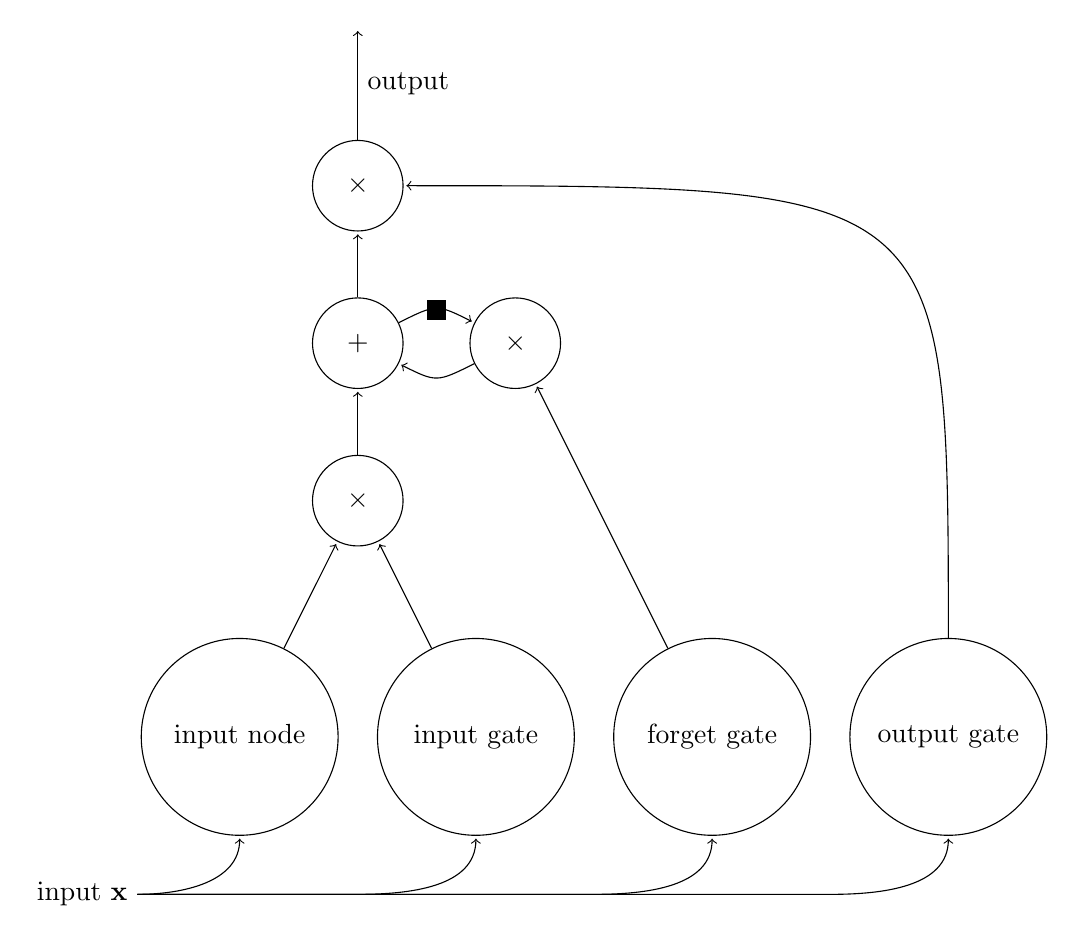
\begin{tikzpicture}[shorten >=1pt]
	\tikzstyle{unit}=[draw,shape=circle,minimum size=1.15cm]
	
	\tikzstyle{gate}=[draw,shape=circle,minimum size=2.5cm]
	
	\node(in) at (0,0) {input $\vec{x}$};
	
	\node[gate](input) at (2,2){input node};
	\node[gate](inGate) at (5,2){input gate};
	\node[gate](forget) at (8,2){forget gate};
	\node[gate](outGate) at (11,2){output gate};
	
	\node[unit](inx) at (3.5,5){$\times$};
	\node[unit](hiddenP) at (3.5,7){$+$};
	
	\node[unit](hidden) at (5.5,7){$\times$};
	\node[unit](outx) at (3.5,9){$\times$};

	
	\draw[->] (in) to[out=0, in=-90] (input);
	\draw[->] (in) to[out=0, in=180] (3.5,0) to[out=0,in=-90] (inGate);
	\draw[->] (in) to[out=0, in=180] (6.5,0) to[out=0,in=-90] (forget);
	\draw[->] (in) to[out=0, in=180] (9.5,0) to[out=0,in=-90] (outGate);
	
	\draw[->] (input) -- (inx);
	\draw[->] (inGate) -- (inx);
	\draw[->] (inx) -- (hiddenP);
	
	\draw[->] (hidden) .. controls (4.5,6.5) .. (hiddenP);
	\draw[->] (hiddenP) .. controls (4.5,7.5) .. (hidden);
	
	\fill[black] (4.375, 7.545) rectangle (4.625,7.295);
	
	\draw[->] (hiddenP) -- (outx);
	
	\draw[->] (forget) -- (hidden);
	\draw[->] (outGate) .. controls (11,9) .. (outx);
	
	\draw[->] (outx) -- (3.5,11) node[midway, right] {output};
	
\end{tikzpicture}
\caption[The cyclic form of an LSTM cell]{The cyclic form of an LSTM cell\footnotemark}
\label{fig:LSTMCell}
\end{figure}

\footnotetext{The rectangle in the cyclic arrow represents a delay of 1 time step.}

\section{Support Vector Machines}
\label{sec:introSVM}


\section{Naive Bayes}
\label{sec:introNB}


\section{Financial Markets}
\label{sec:introFin}

\section{Feature Extraction}
\label{sec:introFeat}

\section{Requirements Analysis}
\label{sec:introReq}


\section{Choice of Tools}
\label{sec:introTool}


\section{Starting Point}
\label{sec:introStart}


\section{Implementation Approach}
\label{sec:introImpl}


\section{Software Engineering Techniques}
\label{sec:introSoft}


\section{Summary}
\label{sec:introSumm}


\chapter{Implementation}

\section{Sentiment Analysis}

\subsection{Data}

\subsubsection{Crawling}

\subsubsection{Pipeline}

\subsection{Features}

\subsection{Multinomial Naive Bayes}

\subsection{Gaussian Naive Bayes}

\subsection{Support Vector Machine}

\section{Price Prediction}

\subsection{Data}

\subsection{Long Short-Term Memory}
\label{sec:ImplLSTM}

\chapter{Evaluation}

\section{Overall Results}

\section{Hyperparameters}

\section{Testing}

\section{Sentiment Evaluation}

\section{Prediction Evaluation}

\section{Summary}

\chapter{Conclusion}

\section{Results}

\section{Lessons Learned}

\section{Further Work}

 
%%%%%%%%%%%%%%%%%%%%%%%%%%%%%%%%%%%%%%%%%%%%%%%%%%%%%%%%%%%%%%%%%%%%%
% the bibliography
\addcontentsline{toc}{chapter}{Bibliography}
\bibliography{refs}


%%%%%%%%%%%%%%%%%%%%%%%%%%%%%%%%%%%%%%%%%%%%%%%%%%%%%%%%%%%%%%%%%%%%%
% the appendices
\appendix

\chapter{Latex source}


\chapter{Project Proposal}

\end{document}